\documentclass[10pt,a4paper,ragged2e]{altacv}


\usepackage[english,russian]{babel}
\usepackage{hyperref}

\geometry{left=2cm,right=10cm,marginparwidth=6.8cm,marginparsep=1.2cm,top=1.25cm,bottom=1.25cm}

\usepackage[utf8]{inputenc}
\usepackage[T1]{fontenc}
\usepackage[default]{lato}

\definecolor{VividPurple}{HTML}{000000}
\definecolor{SlateGrey}{HTML}{2E2E2E}
\definecolor{LightGrey}{HTML}{2E2E2E}
\colorlet{heading}{VividPurple}
\colorlet{accent}{VividPurple}
\colorlet{emphasis}{SlateGrey}
\colorlet{body}{LightGrey}

\renewcommand{\itemmarker}{{\small\textbullet}}
\renewcommand{\ratingmarker}{\faCircle}

\begin{document}
\name{Maxim Filonov}
\personalinfo{%
  \email{max.pengwyn@gmail.com}
  \github{\href{https://github.com/sl1depengwyn}{GitHub}}
  \printinfo{\faTelegram}{\href{https://t.me/sl1depengwyn}{Telegram contact}}
}

\begin{fullwidth}
  \makecvheader
\end{fullwidth}

\AtBeginEnvironment{itemize}{\small}

\cvsection[page1sidebar-eng]{Experience}
\cvevent{Elixir Developer}{\href{https://www.blockscout.com/}{Blockscout}}{Nov 2022 -- Ongoing}
\begin{itemize}
\item Job description 1
\item Job description 2
\end{itemize}

\cvsection{Projects}
\cvproject{Elixireum}
\begin{itemize}
  \item Programming language for smart contracts development on Ethereum built with Elixir.
  \item \href{https://github.com/sl1depengwyn/elixireum}{GitHub}
\end{itemize}
\smallskip
\cvproject{App for report generating}
\begin{itemize}
  \item Application for Windows and Android for \newline \url{https://nadip.ru/} built with Flutter.
\end{itemize}
\smallskip
\cvproject{Parser from EOLANG to JavaScript}
\begin{itemize}
  \item Parser is built using XML и XSLT.
  \item \href{https://github.com/YeslieSnayder/eo}{GitHub}
\end{itemize}
\smallskip
\cvproject{Script for auto-withdrawal of tokens from an address on the Ethereum}
\begin{itemize}
  \item Withdraw tokens from known address as they appear there.
  \item Python with Web3, notifications about withdrawal via bot in Telegram.
\end{itemize}
\smallskip
\cvproject{\href{https://t.me/Coachfood_bot}{Coachfood bot}}
\begin{itemize}
  \item Telegram bot that creates meal plans built with Python using aiogram.
\end{itemize}
\smallskip
\cvproject{\href{https://t.me/drink_enough_bot}{Haskell Telegram bot}}
\begin{itemize}
  \item Lets you know how much we drink. Some interesting features are: customized inline keyboard and visual statistics in the form of graphs.
  \item \href{https://github.com/sl1depengwyn/drink-bot}{GitHub}
\end{itemize}
\smallskip
\cvproject{API for the bot above}
\begin{itemize}
  \item API built with Haskell and Servant
  \item \href{https://github.com/sl1depengwyn/drink-bot-api}{GitHub}
\end{itemize}
\smallskip
\cvproject{Backend for the application that control the robot}
\begin{itemize}
  \item An application written in C++, with an interface made using Qt, which controls a robot with a parallel cable drive. An approximate diagram of the robot:
  \item 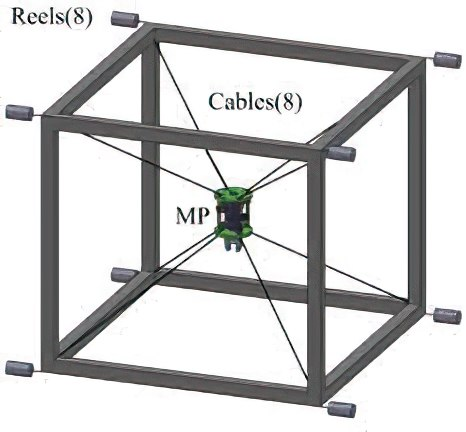
\includegraphics[scale=0.3]{Cube.jpg}
\end{itemize}
\smallskip

\cvsection{Profiles}
\cvproject{\href{https://github.com/sl1depengwyn}{GitHub}}
\smallskip
\cvproject{\href{http://codeforces.com/profile/Pengwyn}{Codeforces}}
\smallskip
\cvproject{\href{https://www.codewars.com/users/Pengwyn1}{Codewars}}
\smallskip

\clearpage

\nocite{*}

\end{document}
